\chapter{The Optimization Problem}\label{chapter:3}

In this chapter we formulate the main optimization problem and introduce the Riemannian conjugate gradient method used to solve it. {\color{red}Additionally, we examine the structure of the initial conditions including the Taylor Green Vortex, and two optimized initial conditions from the results of \cite{zhao_systematic_2023}.}

\section{Formulation of the Problem}

With our initial condition and blowup criterion defined by Theorem \ref{thm:Theorem:1.3}, we now construct the PDE-constrained optimization problem. We begin with the objective functional $\pat: V\rightarrow \RR^+$, which is defined as
\begin{subequations}\label{eq:objective:functional}
\begin{align}
\pat(\bea) &:= \|\nabla \ua(T;\bea)\|_{L^2}^2,\label{eq:objective:functional:1}\\
&\,= \|\ua(T;\bea)\|_{\hdo}^2,\label{eq:objective:functional:2}
\end{align}
\end{subequations}
where $\ua(T;\bea)$ is the solution of the Euler-Voigt equations (\ref{eq:Euler:Voigt}) obtained at the end of the time interval of size $T$ with the initial condition $\bea\in V$ and regularization parameter $\alpha$. Using this objective functional, we define the optimization problem.
\begin{prb}\label{eq:problem}
Given $\alpha, T\in\mathbb{R}^+$, find
\begin{equation}
\tilde{\be}_{\alpha,T} = \argmax_{\beza \in M_C}\pat(\beza),
\end{equation}
\end{prb}
\noindent where $\beza$ is our initial guess. Our goal is to first fix $T$ and solve the optimization problem for a sequence of decreasing values of $\alpha$ that converge to 0. 
From Figure 1b of \cite{bustamante_interplay_2012}, the expected time of singularity formation in the Euler flow, with the TGV scaled as discussed in Section \ref{sec:scaling} used as the initial condition, is $T^*\approx 4$. From Theorem \ref{thm:Theorem:1.3}, if the initial condition criterion (\ref{eq:eta:0:condition}) and objective functional criteria (\ref{eq:alpha:sup}) are both satisfied, then the corresponding Euler flow develops a singularity in the interval $[0,T^*]$ from initial condition $\be$. We examine the results for a time interval slightly shorter and longer than $T^*$. Therefore, we consider the optimization problem for $T=3$, and $T=5$. With optimization, blow-up may occur in both cases. {\color{red}All regularization parameters used in this analysis are a fraction $\alpha=\cdot/1024$. In order to simplify the notation of our optimal solution, we drop the denominator, i.e., the optimal initial condition found by solving problem (\ref{eq:problem}) for regularization parameter $\alpha=8/1024$ and time interval $T=5$ would be denoted $\tilde{\be}_{8,5}$.}

\section{Initial Guesses}

Problem \ref{eq:problem} is non-convex and so may admit a different local maxima depending on the initial guess used at iteration zero, $\beza$. In order to search for optimal initial conditions that may lead to a singularity in the Euler flow, we must solve the optimization problem from different initial guesses. Before we begin our search for singularities, we examine the structure of the initial guesses used in this study. These include the TGV as well as two optimal initial conditions from the results of \cite{zhao_systematic_2023}.
\\~\\
Figure \ref{fig:TGV:Init} shows the isosurfaces of the magnitude of the vorticity {\color{red}$\w = \bn\times\be_{TGV}$. In \cite{zhao_systematic_2023}, the authors utilized the Riemannian conjugate gradient method to identify initial conditions that produce 'extreme' behaviour in Euler flows. Their analysis used the same domain $\Omega$ as our analysis. However, the manifold in which they searched for optimal initial conditions was formulated by scaling the initial conditions to a fixed $\|\be\|_{\hdt} = 1$ and the objective functional was $\Phi_T(\be) := \|\u(T;\be)\|_{\hdt}^2$. With the same domain size $L=1$, this gives their initial conditions a time interval which is scaled by a factor of $6\sqrt{3}\pi^2$ to our model, which is shown in Appendix \ref{app:tg:seminorm:general}. They solved the optimization problem with multiple initial guesses, including the TGV, and time intervals of $T=25$ and $T=75$. In our manifold (\ref{eq:manifold}), this is equivalent to starting from the TGV and optimizing with time intervals of $T\approx 0.2437$ and $T\approx 0.7312$, respectively. The first initial condition from \cite{zhao_systematic_2023} is the optimal initial condition found using the short time window $T=25$ and a resolution of $N=128^3$. We denote this initial condition as $\be_{S}$. Figure \ref{fig:XS:Init} shows the isosurfaces of the magnitude of the vorticity for $\be_{S}$. The second is the optimal initial condition found using the long time window $T=75$ and a resolution of $N=512^3$, which we denote as $\be_{L}$. Figure \ref{} shows the isosurfaces of the magnitude of the vorticity for $\be_{L}$.
}
\begin{figure}[h!]
\centering
\begin{subfigure}{.4\textwidth}
  \centering
  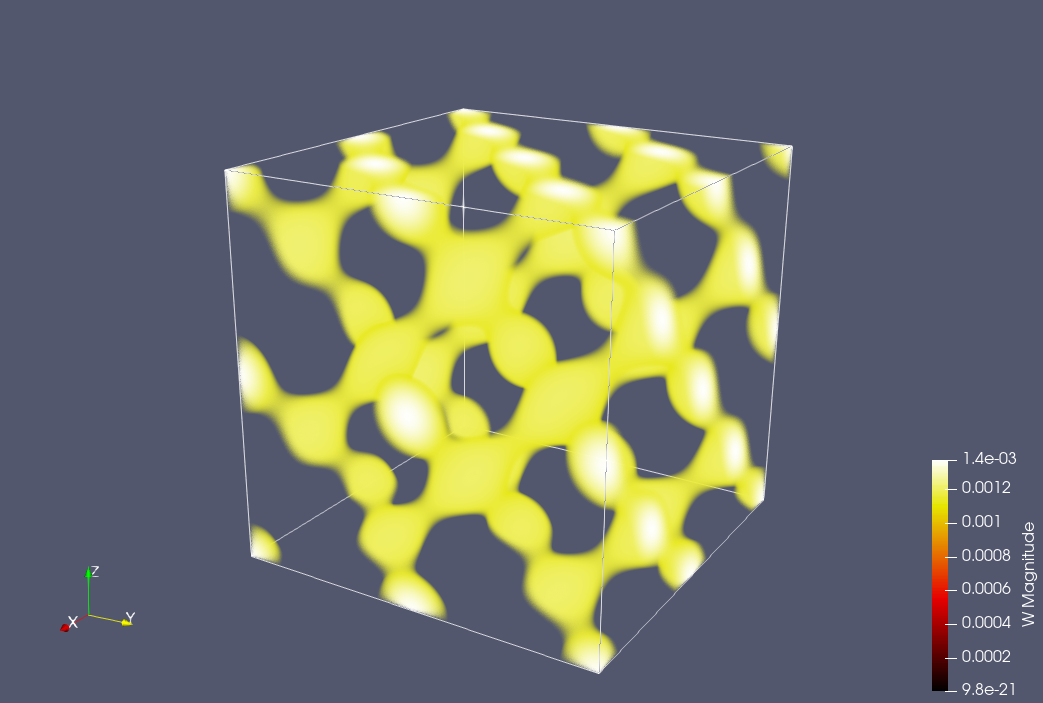
\includegraphics[width=.9\linewidth]{../../results/Final_Results/Visualizations/TGV_M.png}
  \caption{}
  \label{fig:sub1}
\end{subfigure}%
\begin{subfigure}{.4\textwidth}
  \centering
  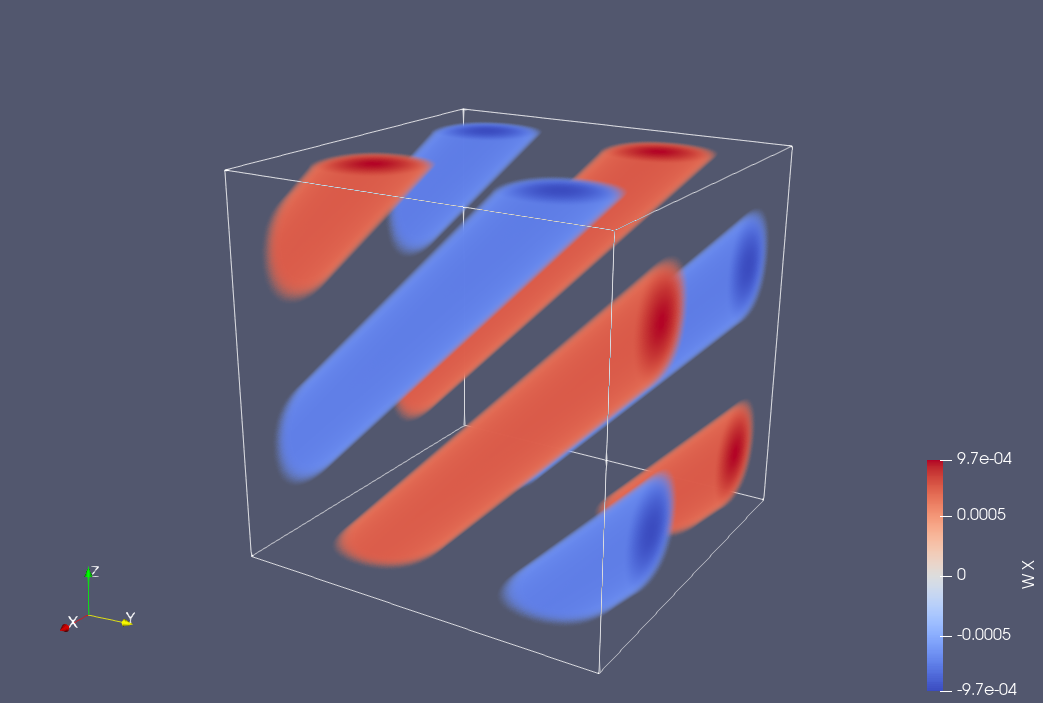
\includegraphics[width=.9\linewidth]{../../results/Final_Results/Visualizations/TGV_X.png}
  \caption{}
  \label{fig:sub2}
\end{subfigure}
\\
\begin{subfigure}{.4\textwidth}
  \centering
  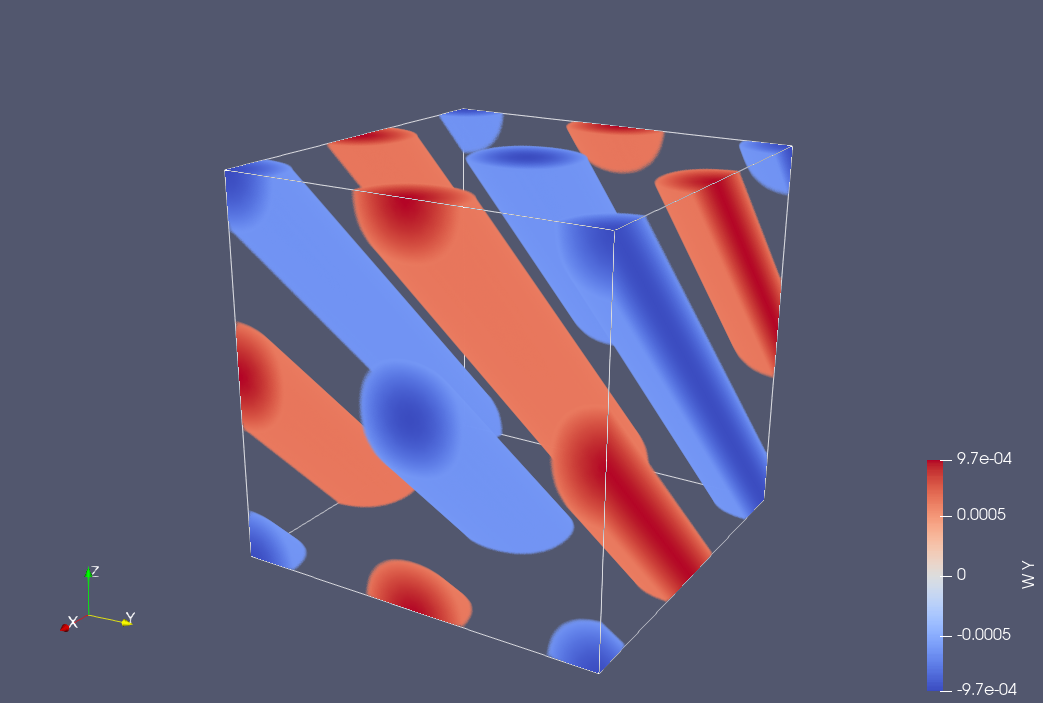
\includegraphics[width=.9\linewidth]{../../results/Final_Results/Visualizations/TGV_Y.png}
  \caption{}
  \label{fig:sub1}
\end{subfigure}%
\begin{subfigure}{.4\textwidth}
  \centering
  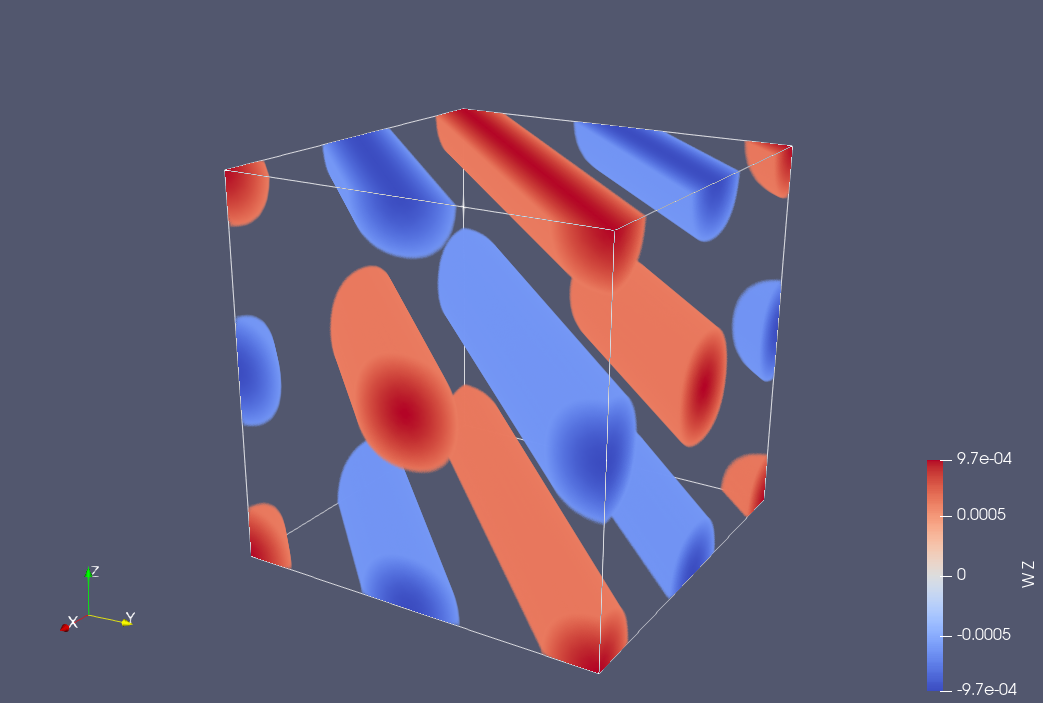
\includegraphics[width=.9\linewidth]{../../results/Final_Results/Visualizations/TGV_Z.png}
  \caption{}
  \label{fig:sub2}
\end{subfigure}
\caption{Isosurfaces of vorticity $\omega=\bn \times \be_{TGV}$ (a) magnitude $|\w(\x)|$, and components (b) $|\omega_1|$, (c) $|\omega_2|$, and (d) $|\omega_3|$.}
\label{fig:TGV:Init}
\end{figure} 

\begin{figure}[h!]
\centering
\begin{subfigure}{.4\textwidth}
  \centering
  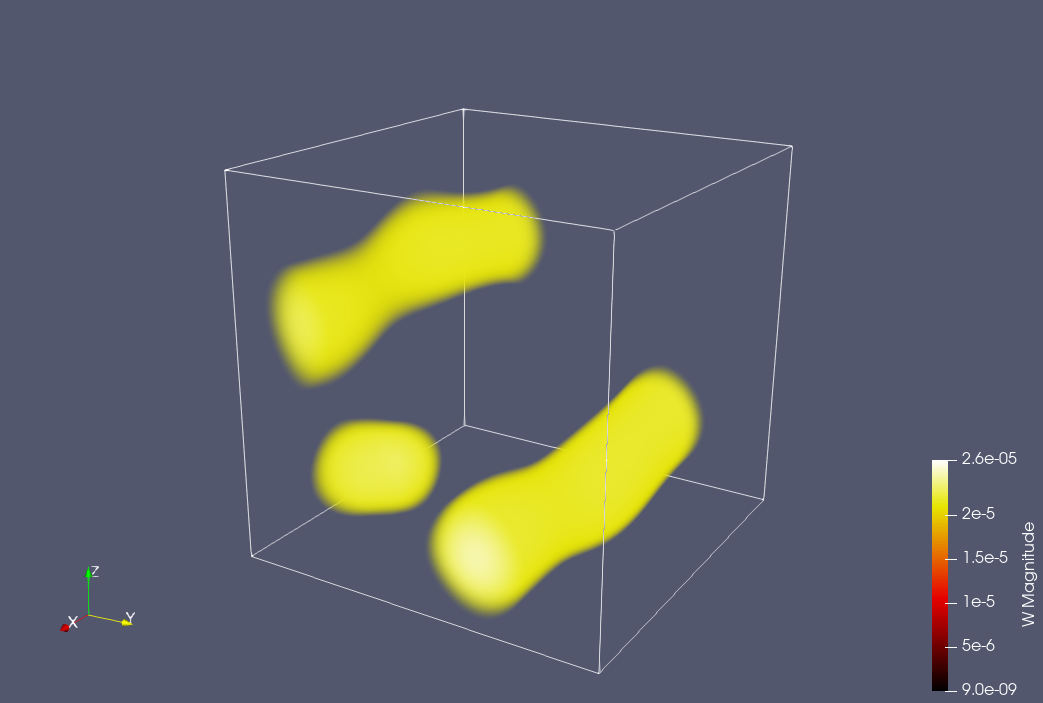
\includegraphics[width=.9\linewidth]{../../results/Final_Results/Visualizations/XS_M.png}
  \caption{}
  \label{fig:sub1}
\end{subfigure}%
\begin{subfigure}{.4\textwidth}
  \centering
  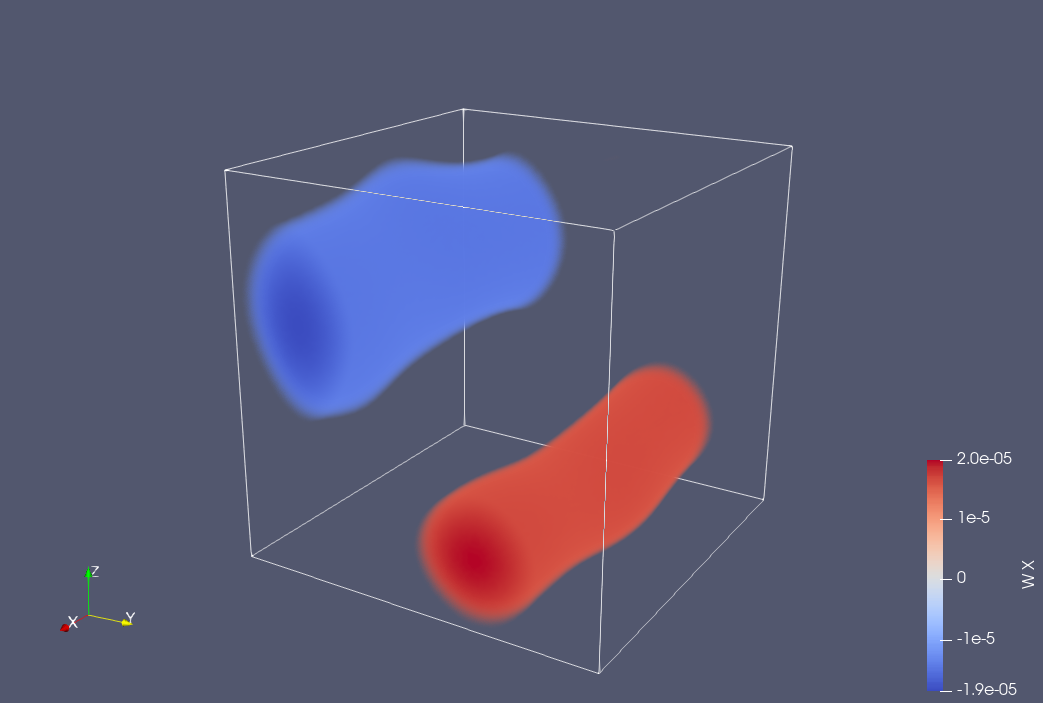
\includegraphics[width=.9\linewidth]{../../results/Final_Results/Visualizations/XS_X.png}
  \caption{}
  \label{fig:sub2}
\end{subfigure}
\\
\begin{subfigure}{.4\textwidth}
  \centering
  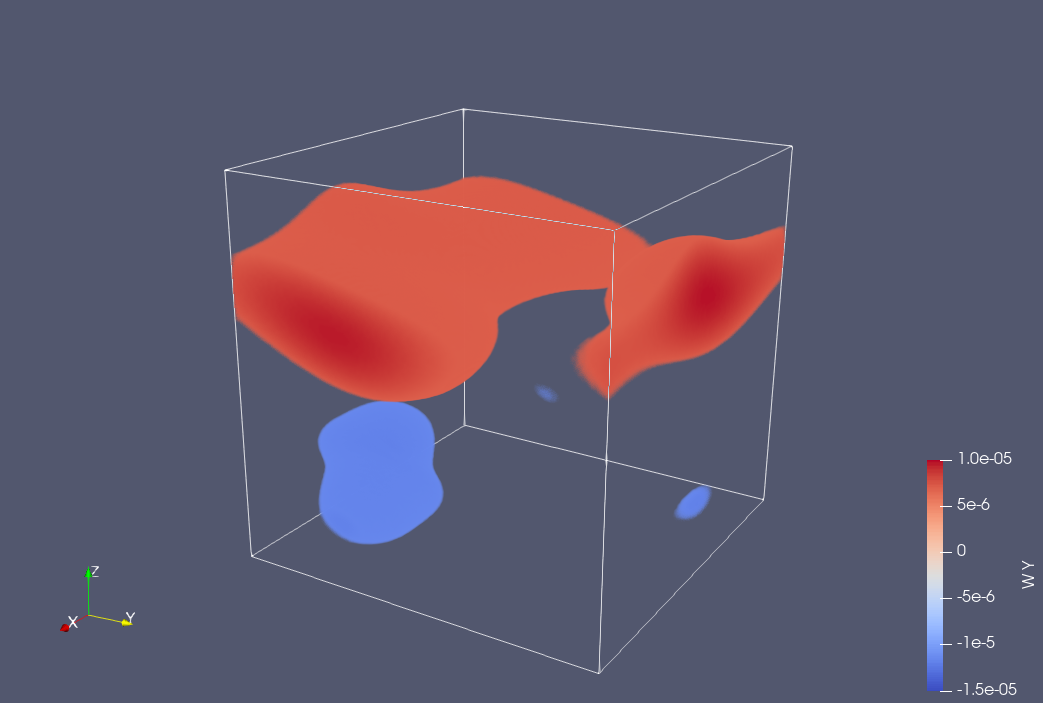
\includegraphics[width=.9\linewidth]{../../results/Final_Results/Visualizations/XS_Y.png}
  \caption{}
  \label{fig:sub1}
\end{subfigure}%
\begin{subfigure}{.4\textwidth}
  \centering
  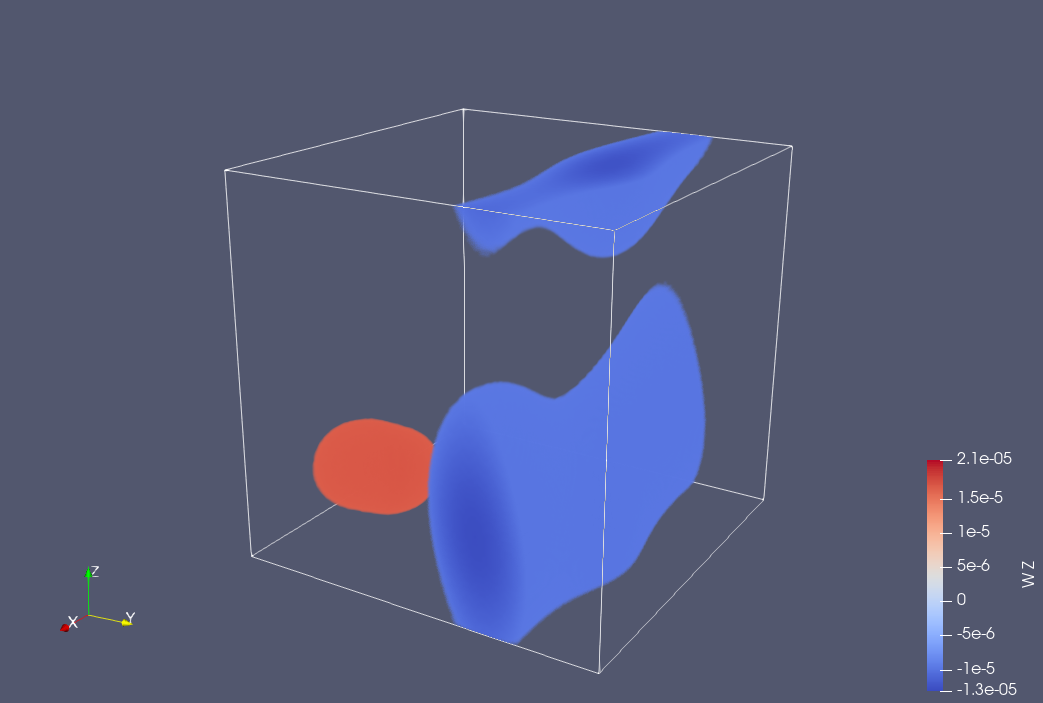
\includegraphics[width=.9\linewidth]{../../results/Final_Results/Visualizations/XS_Z.png}
  \caption{}
  \label{fig:sub2}
\end{subfigure}
\caption{Isosurfaces of vorticity $\omega=\bn \times \be_{S}$ (a) magnitude $|\w(\x)|$, and components (b) $|\omega_1|$, (c) $|\omega_2|$, and (d) $|\omega_3|$.}
\label{fig:XS:Init}
\end{figure}




\section{Gradient of Objective Function} \label{sec:Gateaux Directional Differential}
 
The optimization problem (\ref{eq:problem}) is solved using a Riemannian conjugate gradient method which uses an optimal search direction and distance to create the next approximation of the optimal initial condition. This method is utilized because it accelerates the gradient ascent method which is necessary given the computational cost of each iteration. To solve this problem, we utilize a 'optimize-then-discretize' approach where the optimization problem, and the Riemannian conjugate gradient method, are derived in an infinite-dimensional function space and then discretized to solve numerically. The same method was used in \cite{zhao_systematic_2023} to solve a PDE-constrained optimization problem for the Euler equations to search for initial conditions $\be$ that produce 'extreme' flows. 
\\~\\
We compute the optimal search direction using the gradient of the objection functional $\nabla\pat(\bea)$. It is obtained using an adjoint method which depends on solving a properly defined adjoint system backwards in time. To derive an expression for the gradient, we first introduce the G\^{a}teaux (directional) differential $\ppat(\bea;\bea'): V\times V \rightarrow \mathbb{R}$. The Gateaux differential is defined as,
\begin{align}\label{eq:Gateaux:differential}
\ppat(\bea;\bea'):=\lim_{\epsilon\rightarrow 0}\frac{1}{\epsilon}\left[\pat(\bea+\epsilon\bepa)-\pat(\bea)\right].
\end{align}
This represents the change in $\pat$ from  an infinitesimal perturbation in the direction $\bepa$ from the initial condition $\bea$. By fixing the initial condition $\bea$, we can view the G\^{a}teaux differential as a bounded linear functional on $V$. Therefore, it can also be represented as an inner product on the Gevrey space using the Riesz representation theorem \cite{zhao_systematic_2023,luenberger_optimization_1969}
\begin{equation}\label{eq:Gateaux:differential:riesz}
\ppat(\bea;\bepa) = \la \nabla\pat(\bea),\bepa\ra_{G^\sigma}.
\end{equation}
Substituting the second definition of the objective functional (\ref{eq:objective:functional:2}) into the definition of the G\^{a}teaux differential (\ref{eq:Gateaux:differential}), we derive the G\^{a}teaux differential in the form of the $\hdo$ inner product,
\begin{equation}\label{eq:Gateaux:differential:inner:product}
\ppat(\bea;\bepa) =  2\la \ua(T),\upa(T)\ra_{\hdo}
\end{equation}
The derivation for this is shown in Appendix \ref{app:gateaux}. In (\ref{eq:Gateaux:differential:inner:product}) the value $\upa$ is the solution of the linearization of the Euler-Voigt system (\ref{eq:Euler:Voigt}) around its solution $\ua$ corresponding to the initial condition $\bea$. The linearization of the Euler-Voigt system is defined as\\
\begin{small}
\begin{subequations}\label{eq:euler:voigt:linearization}
\begin{align}
\L\begin{bmatrix}
\upa \\
\ppa
\end{bmatrix} :=& 
\begin{bmatrix}
\partial_t \upa +(I-\alpha^2\Delta)^{-1}(\ua\cdot\bn\upa +\upa\cdot\bn \ua+\bn \ppa)\\
      \nabla\cdot \upa\\
\end{bmatrix} = \begin{bmatrix}
0\\
0
\end{bmatrix}\\
\upa(x,0) =& \bepa
\end{align}
\end{subequations}
\end{small}
\noindent where $\bepa$ and $\ppa$ are the perturbations of the initial condition and pressure, respectively. The derivation of the linearized form of the Euler-Voigt equations is shown in Appendix \ref{app:lin:euler}. In order to obtain the gradient of the objective functional from the G\^{a}teaux differential we must first introduce the fields $\lb \usa, \psa \rb$ which are the solution of the adjoint system
\small
\begin{subequations}\label{eq:euler:voigt:adjoint}
\begin{align}
\L^*\begin{bmatrix}
\usa\\
\psa
\end{bmatrix} :=& \begin{bmatrix}
\text{-}\partial_t\usa\text{-}(\bn (I\text{-}\alpha^2\Delta)^{-1}\usa + (\bn (I\text{-}\alpha^2\Delta)^{-1}\usa)^{\intercal})\ua\text{-}\bn \psa\\
-\bn \cdot \usa
\end{bmatrix} = \begin{bmatrix}
0\\
0
\end{bmatrix}\\
\usa(\x,T) =& 2|D|^2\ua(\x,T)
\end{align}
\end{subequations}
\normalsize
which is derived in Appendix \ref{app:adjoint} by performing integration by parts, in both space and time, on the following duality-pairing relation 
\begin{equation}\label{eq:duality:pairing}
\begin{aligned}
\left(\L\begin{bmatrix}
\upa\\
\ppa
\end{bmatrix}, \begin{bmatrix}
\usa\\
\ppa
\end{bmatrix} \right) :=& \int_0^T\int_{\TT^3} \L\begin{bmatrix}
\upa\\
\ppa
\end{bmatrix}, \begin{bmatrix}
\usa\\
\psa
\end{bmatrix} \,d\x\,dt \\[3pt]
=& \left( \begin{bmatrix}
\upa\\
\ppa
\end{bmatrix},\L^*\begin{bmatrix}
\usa\\
\psa
\end{bmatrix} \right) + \int_{\TT^3} \upa(\x,T)\cdot \usa(\x,T)\,d\x \\[3pt]
&- \int_{\TT^3}\upa(\x,0)\cdot \usa(\x,0) \,d\x \\
=& \, 0.
\end{aligned}
\end{equation}
Using the solutions of the adjoint system we can now obtain a convenient expression for the gradient. With the G\^{a}teaux differential (\ref{eq:Gateaux:differential:inner:product}) expressed in terms of the $L^2$ inner product 
\begin{equation}\label{eq:Gateaux:differential:inner:product:2}
\ppat(\bea;\bepa) = \la \usa(0),\upa(0)\ra_{L^2},
\end{equation}
which is derived in Appendix \ref{app:gateaux}, and in the Riesz representation form (\ref{eq:Gateaux:differential:riesz}), we obtain
\begin{equation}
\ppat(\bea;\bepa) = \la \usa(0),\upa(0)\ra_{L^2} = \la \nabla\pat(\bea),\bepa \ra_{G^\sigma}.
\end{equation}
Using the definition of the Gevrey inner product (\ref{eq:Gevrey:Inner:Product}), the $L^2$ inner product can be converted to the Gevrey inner product,
\begin{equation}
\la \usa(0),\upa(0)\ra_{L^2} = \la (1+|D|^2)^{-3}e^{-2\sigma|D|} \usa(0),\bepa \ra_{G^\sigma}.
\end{equation}
Therefore, we have two forms of the G\^{a}teaux differential as a Gevrey inner product
\begin{equation}
\ppat(\bea;\bea') = \la \nabla\pat(\bea),\bepa \ra_{G^\sigma} = \la (1+|D|^2)^{-3}e^{-2\sigma|D|} \usa(0),\bepa \ra_{G^\sigma}.
\end{equation}
From this we obtain the gradient of the objective functional
\begin{equation}\label{eq:gradient}
\nabla \pat(\bea) = (1+|D|^2)^{-3}e^{-2\sigma|D|}\usa(0).
\end{equation}
The adjoint system (\ref{eq:euler:voigt:adjoint}) is linear and represents a terminal value problem. Its coefficients are determined by evolving the Euler-Voigt system forward from the initial condition $\bea$ to compute $\ua(T)$, from which we obtain the terminal value of (\ref{eq:euler:voigt:adjoint}). Finally, we evolve the adjoint system backwards in time to obtain the initial value $\usa(0)$ which is used to compute the gradient (\ref{eq:gradient}).

\section{Riemannian Conjugate Gradient Method}\label{sec:Riemannian Conjugate Gradient Method}

When solving the optimization problem, we look for an initial condition $\bea \in M_C$ that maximizes our objective functional. Therefore, not only must our initial guess $\beza$ have a $\hdo$ seminorm of $\sqrt{3}/2$, but so too must each following iterate $\bena$. We ensure this constraint is satisfied using a Riemannian conjugate gradient method modified from the method used in \cite{danaila_computation_2017,protas_systematic_2022,zhao_systematic_2023}. This method has three steps: 
\begin{enumerate}
  \item Project the gradient $\nabla\Phi_T(\bea)$ onto the tangent space to $\M_C$ at $\bea$.
  \item Perform a suitable vector transport operation in order to construct a Riemannian conjugate ascent direction using the previous search direction.
  \item Retract the resulting state back to the constraint manifold $\M_c$.
\end{enumerate}
We first define the space tangent to $\M_C$ at $\v$ as
\begin{equation}\label{eq:tangent:space}
T_{\v}\M_C = \lb \z\in V : \la \v,\z\ra_{\hdo}=0\rb.
\end{equation}
For any $\z\in \T_{\v}\M_C$, this condition can be expressed as
\begin{subequations}
\begin{align}
\la \v,\z\ra_{\hdo} &= \int_{\TT^3}|D|\v\cdot|D|\z d\x \\
&= \int_{\TT^3} (1+|D|^2)^3e^{2\sigma|D|}\left((1+|D|^2)^{-3}e^{-2\sigma|D|}|D|^2\v\right)\cdot\z \,d\x \\
&= \la (1+|D|^2)^{-3}e^{-2\sigma|D|}|D|^2\v,\z\ra_{G^\sigma} = 0.
\end{align}
\end{subequations}
Thus, at each point $\v\in M_C$, the tangent space $\T_{\v}\M_C$ can be characterized using the unit 'normal' vector given by 
\begin{equation}
\n_{\v} = \frac{(1+|D|^2)^{-3}e^{-2\sigma|D|}|D|^2\v}{\|(1+|D|^2)^{-3}e^{-2\sigma|D|}|D|^2\v\|_{G^\sigma}}
\end{equation}
which allows us to construct the projection operator $\P_{\T_{\v}M_C}: V \rightarrow \T_{\v}\M_C$, 
\begin{equation}\label{eq:projection:operator}
\forall \w \in V, \quad \P_{\T_{\v}\M_C}\w = \w - \la \n_{\v}, \w \ra_{G^\sigma}\n_{\v}.
\end{equation}
As stated previously, the initial conditions at each iteration must have a $\hdo$ seminorm of $\sqrt{3}/2$. In order to ensure this we introduce the retraction operator
\begin{equation}\label{eq:retraction:operator}
R(\v) = \frac{\sqrt{3}}{2}\frac{\v}{\|\v\|_{\hdo}}, \qquad \v\neq \boldsymbol 0.
\end{equation}
The conjugate-gradient method method uses the search direction obtained at the $n$-th iteration to compute the search direction at the $(n+1)$-th iteration. This is done by computing a linear combination of the gradient at the current iteration and the search direction from the previous iteration, weighted with a 'momentum' coefficient. However, the two directions belong to different tangent spaces to $\M_C$ and thus cannot be directly added. In order to allow algebraic operations to be performed on the vectors of the two tangent spaces we introduce the vector transport operation defined by \cite{absil_optimization_2008}
$$\T\M_C \oplus \T\M_C \rightarrow \T\M_C \quad:\quad (\bp,\bx)\mapsto \Gamma_{\bp}(\bx)\in \T\M_C, $$
where $\T\M_C = \bigcup_{\v\in\M_C}\T_{\v}\M_C$ is the tangent bundle on $\M_C$. The operation transports the vector field $\bx$ along the manifold $M_C$ in the direction of $\bp$. This allows us to map search directions between the tangent spaces of two consecutive iterations. This operator is defined via differentiated retraction
\begin{subequations}\label{eq:vector:transport}
\begin{align}
\Gamma_{\varphi_{\u}}(\xi_{\u}) &:= \frac{d}{dt} R(\varphi_{\u} + t\xi_{\u})\big|_{t=0}\\
&:= \frac{\sqrt{3}}{2} \frac{1}{\|\u+\varphi_{\u}\|_{\hdo}} \left[\xi_{\u} - \frac{\la \u+\varphi_{\u},\xi_{\u}\ra_{\hdo}}{\|\u + \varphi_{\u}\|_{\hdo}^2}(\u + \varphi_{\u})\right],\quad \u\in M_C.
\end{align}
\end{subequations}
\noindent With our operators defined we can now construct the iterative relation that will be used to maximization our objective functional (\ref{eq:objective:functional})
\begin{equation}\label{eq:iteration}
\benpa = R\left[\bena + \tau_n \d^{(n)}\right].
\end{equation}
To simply notation, let $\bds G^{(n)} := \nabla\pat(\bena)$ and let $\T_n := \T_{\bena}\M_C$. The search direction at iteration $n$ ($\d^{(n)}$) is computed as
\begin{small}
\begin{subequations}\label{eq:search:direction}
\begin{align*}
\d^{(0)} &= P_{\T_0}\bds G^{(0)} \\
\d^{(n)} &= P_{\T_n}\bds G^{(n)} + \beta_n\Gamma_{\tau_{n-1}\d^{(n-1)}}(\d^{(n-1)}), \quad n\geq 1,
\end{align*}
\end{subequations}
\end{small}
where the 'momentum' term is computed using the Polak-Ribi$\grave{\text{e}}$re approach \cite{nocedal_numerical_2000}.
\begin{small}
\begin{equation}
\beta_n = \frac{\la P_{\T_n}\bds G^{(n)}, \left( P_{\T_n}\bds G^{(n)} - \Gamma_{\tau_{n-1}\d^{n-1}}P_{\T_{n-1}} \bds G^{(n-1)} \right) \ra_{G^\sigma}}{\|P_{\T_{n-1}} \bds G^{(n-1)}\|_{G^\sigma}^2}.
\end{equation}
\end{small}
\noindent In order to remove old data that may slow down convergence, the algorithm is periodically restarted by setting $\beta_n = 0$. For our optimization search, we restart the algorithm every 20 iterations, and when the search direction is not an ascent direction, i.e, when
\begin{equation}
\frac{\la \d^{(n)},P_{\T_n}G^{(n)} \ra_{G^\sigma}}{\|\d^{(n)}\|_{G^\sigma}\|P_{\T_n}G^{(n)}\|_{G^\sigma}} < 0.
\end{equation}
Finally, our optimal step size is determined by the distance along an arc tangent to $\d^{(n)}$ which maximizes the objective functional, it is computed by performing an arc-search along this direction using a modification of Brent's method
\begin{equation}\label{eq:step:size}
\tau_n = \argmax_{\tau > 0} \Phi_T\left( R\left[ \eta^{(n)} + \tau \d^{(n)} \right] \right).
\end{equation}
The optimization search is terminated when the relative change in the objective functional from (\ref{eq:iteration}) is below a chosen tolerance.
\begin{equation}\label{eq:stop}
0 \leq \frac{\pat(\benpa)-\pat(\bena)}{\pat(\bena)} < tol,
\end{equation}
where $tol = 10^{-10}$. {\color{red}The complete optimization search algorithm is summarized in Algorithm \ref{alg:opt}.


\begin{algorithm}
\caption{Solution of Problem \ref{eq:problem} for initial guess $\beza$ and fixed $\alpha$ and $T$.}\label{alg:opt}

\,\\
\textbf{Input:} \\
\hspace*{\algorithmicindent} $\alpha$ - regularization parameter\\
\hspace*{\algorithmicindent} $T$ - length of time interval\\
\hspace*{\algorithmicindent} $\beza$ - initial guess\\
\hspace*{\algorithmicindent} $N$ - resolution\\
\hspace*{\algorithmicindent} $n$ - iteration number\\
\textbf{Output:}\\
\hspace*{\algorithmicindent} $\beat$ - optimal initial condition\\
\hrule

\begin{algorithmic}

\State $n \gets 0$
\While{(\ref{eq:stop}) is not satisfied}\\
\hspace*{\algorithmicindent} Solve the Euler-Voigt system with initial condition $\bena$, see equation (\ref{eq:Euler:Voigt})\\
\hspace*{\algorithmicindent} Solve the adjoint system to obtain $\usa$ and $p^*$, see equation (\ref{eq:euler:voigt:adjoint}) \\
\hspace*{\algorithmicindent} Compute the gradient $\bn \pat(\bena)$, see equation (\ref{eq:gradient}) \\
\hspace*{\algorithmicindent} Compute the search direction $\d^{(n)}$, see equation (\ref{eq:search:direction}) \\
\hspace*{\algorithmicindent} Compute the optimal step size $\tau_n$, see equation (\ref{eq:step:size}) \\
\hspace*{\algorithmicindent} Compute the next optimal initial condition $\benpa$, see equation (\ref{eq:iteration}) \\
\hspace*{\algorithmicindent} $n \gets n+1$

\EndWhile\\

$\beat \gets \bena$ \\~\\

\hrule

\If{the flow corresponding to $\beat$ is under-resolved, see equation (\ref{eq:spectrum})} \\
\hspace*{\algorithmicindent} $N \gets 2N$ \\
\hspace*{\algorithmicindent} $\beza \gets \beat$ \\
\hspace*{\algorithmicindent} Repeat Algorithm \ref{alg:opt}

\EndIf

\end{algorithmic}


\end{algorithm}
}


